\documentclass{exam}
\usepackage[utf8]{inputenc}
\usepackage{upgreek}
\usepackage[margin=1in]{geometry}
\usepackage{amsmath,amssymb}
\usepackage{multicol}
\usepackage{stmaryrd}
\usepackage{graphicx}
\usepackage{caption}
\usepackage{tikz}
\usepackage{dsfont}
\usepackage{enumitem}
\usepackage{hyperref}
\usetikzlibrary{matrix}
\newcommand\tab[1][1cm]{\hspace*{#1}}
\pagestyle{head}
\firstpageheader{}{}{}
\runningheader{\examnum}{\class}{\name}
\runningheadrule
\newcommand{\class}{Fundamentos de bases de datos}
\newcommand{\term}{Facultad de Ciencias UNAM}
\newcommand{\examnum}{Tarea 04}
\newcommand{\examdate}{06/05/2022}
\newcommand{\name}{Jurassic Team}

\def\ojoin{\setbox0=\hbox{$\bowtie$}%
  \rule[-.02ex]{.25em}{.4pt}\llap{\rule[\ht0]{.25em}{.4pt}}}
\def\leftouterjoin{\mathbin{\ojoin\mkern-5.8mu\bowtie}}
\def\rightouterjoin{\mathbin{\bowtie\mkern-5.8mu\ojoin}}
\def\fullouterjoin{\mathbin{\ojoin\mkern-5.8mu\bowtie\mkern-5.8mu\ojoin}}

\begin{document}

\noindent
\begin{tabular*}{\textwidth}{l @{\extracolsep{\fill}} r @{\extracolsep{6pt}} l}
\textbf{\class} & \textbf{\term}\\
\textbf{\examnum} & \textbf{\name}\\
\textbf{\examdate}
\end{tabular*}\\
\rule[2ex]{\textwidth}{2pt}

\section*{Preguntas}
%AQUI VAN LAS PREGUNTAS
\begin{questions}
	\question \textbf{Cardinalidad de la consulta}\\
	Considera las siguientes relaciones:\\
	\begin{figure}[h!]
		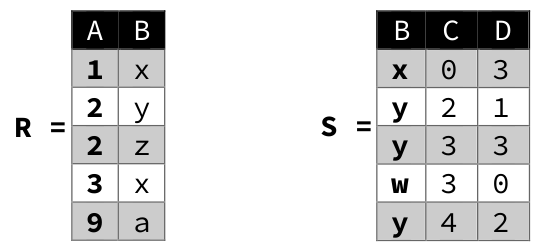
\includegraphics[width=7cm]{imgs/1.png}
		\centering
	\end{figure}	\\
	Para las siguientes expresiones de \textbf{álgebra relacional}, completa la tabla con el número de tuplas que cada una de ellas
produce utilizando las relaciones \textbf{R} y \textbf{S}.\\
	\begin{figure}[h!]
		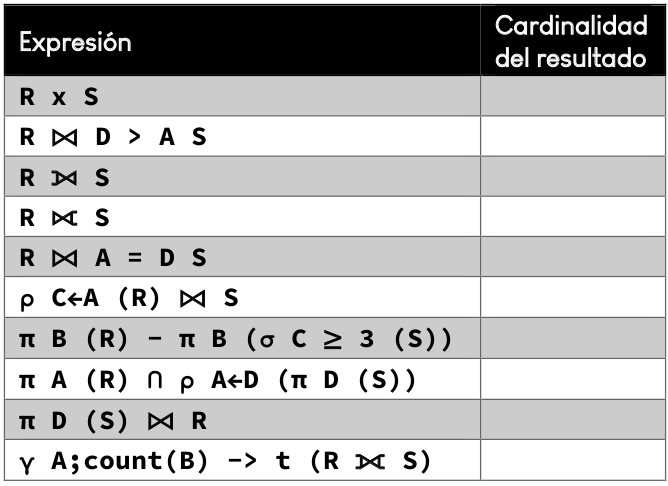
\includegraphics[width=9cm]{imgs/1.1.png}
		\centering
	\end{figure}	
	
	\newpage
	\question \textbf{Banco del Sur}\\
	Tienes el siguiente \textbf{esquema de una base de datos} para una institución bancaria \textbf{utilizado en los videos}:\\
	\begin{figure}[h!]
		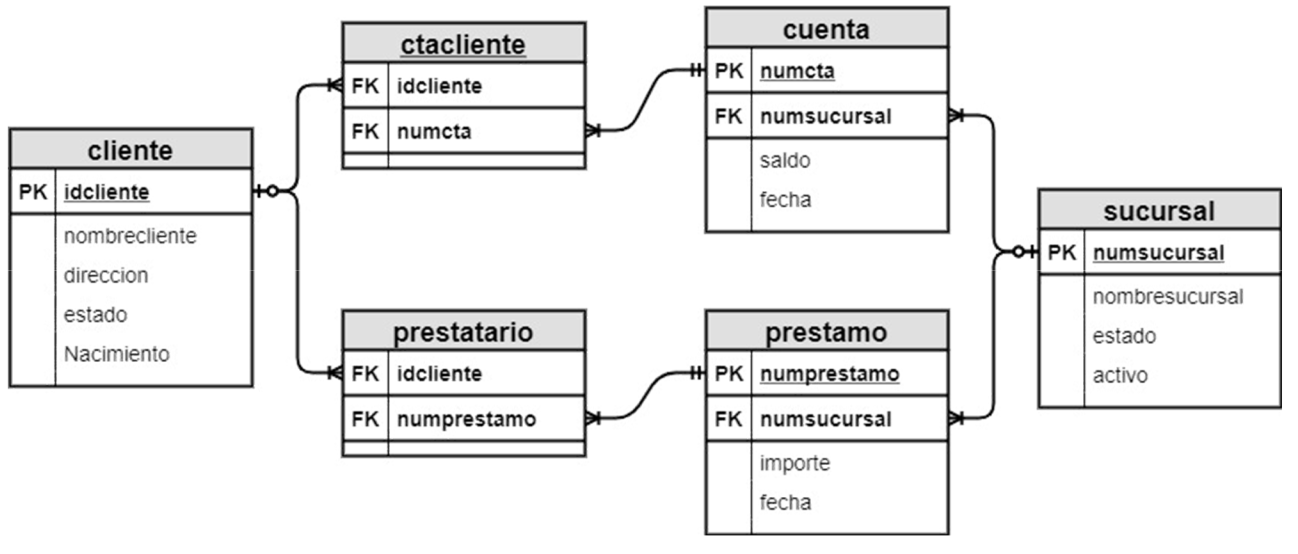
\includegraphics[width=15cm]{imgs/2.png}
		\centering
	\end{figure}	\\
	Escribe una \textbf{expresión de álgebra relacional} para responder las siguientes consultas. Deberás comprobar cada una ellas
en la calculadora \textbf{Relax} y agregar en cada inciso una la \textbf{expresión} y una \textbf{captura de pantalla} con el resultado obtenido:
	
	\begin{enumerate}[label=\alph*.]
		\item Obtener toda la información de los clientes que viven en \textbf{QUINTANA ROO}, que hayan nacido entre el \textbf{19 de septiembre
de 1983} y el \textbf{21 de septiembre de 1986} que tengan algún \textbf{préstamo} entregado durante \textbf{2014}. Mostrar la información
\textbf{ordenada} por el \textbf{nombre del cliente}.
		\item Obtener una relación de los clientes que \textbf{tienen una cuenta} con un saldo entre \textbf{\$85,000.00} y \textbf{\$115,000.00}, pero que \textbf{no tienen ningún préstamo} en el banco. Mostrar el \textbf{idcliente}, \textbf{nombre del cliente}, \textbf{número de cuenta} y \textbf{saldo}.
		\item Obtener el \textbf{nombre} de todos los clientes que tienen \textbf{un préstamo} y el \textbf{importe} de este. El \textbf{importe} debe ser mayor de \textbf{\$95,000} y se debió entregar durante el \textbf{segundo trimestre de 2014} en el estado de \textbf{OAXACA}.
		\item Toda la información de las sucursales con clientes que tengan un préstamo otorgado en el banco en alguna de las sucursales de \textbf{YUCATÁN} y que no vivan en \textbf{NAYARIT}.
		\item Toda la información de los clientes que solo tiene algún \textbf{préstamo} (ninguna cuenta) entregado en el \textbf{primer trimestre de 2013} y aquellos que solo tienen alguna \textbf{cuenta} (ningún préstamo) entregada durante el \textbf{segundo trimestre de 2014}.
		\item Una lista que muestre el \textbf{estado}, el \textbf{nombre de la sucursal} y el \textbf{total de clientes} que se tienen, considerando que los clientes deben tener una \textbf{cuenta} con saldo entre \textbf{\$90,000} y \textbf{\$120,000}, entregada en \textbf{2012} o \textbf{2014}.
		\item Información de los clientes con \textbf{saldo} entre \textbf{\$30,000.00} y \textbf{\$45,000.00} que vivan no vivan en \textbf{GUERRERO} y que no han solicitado ningún \textbf{préstamo}.
		\item Una lista con el \textbf{saldo promedio, mayor saldo, menor saldo, y total de cuentas}, por \textbf{estado} y \textbf{sucursal}. El \textbf{saldo promedio} debe ser \textbf{mayor} que \textbf{\$80,000.00} y \textbf{menor} que \textbf{\$100,000.00} de los estados de \textbf{TABASCO, YUCATÁN Y QUINTANA ROO}.
		\item El estado que ha otorgado la \textbf{menor cantidad de préstamos}, cuyo importe esté entre \textbf{\$75,000.00} y \textbf{\$90,000.00}. Se debe mostrar también el \textbf{total de préstamos} que haya entregado.
		\item El \textbf{id}, \textbf{nombre del cliente}, \textbf{sucursal} y \textbf{saldo} de aquel cliente que tenga el \textbf{mayor importe} de todos los préstamos del
banco.
	\end{enumerate}
	
	\textbf{Operaciones de mantenimiento de datos: borrado, inserción y actualización}
	\begin{enumerate}[label=\alph*.]
		\item Borrar toda la información del cliente \textbf{EDMUNDO RUBIO MONTERO}.
		\item Borrar todas las cuentas de la sucursal \textbf{CHILPANCINGO} con un \textbf{saldo} entre \textbf{\$75,000.00} y \textbf{\$90,000.00}.
		\item Ofrecer un nuevo préstamo con \textbf{\$20,000.00} a todos los clientes que tienen cuenta con saldo mayor de \textbf{\$60,000.00} y menor de \textbf{\$75,000.00} en la sucursal \textbf{BONAMPAK}, el número del nuevo préstamo será el de la cuenta que poseen. A los clientes con un saldo es mayor o igual a \textbf{\$75,000.00}, se les otorgará un préstamo de \textbf{\$30,000.00}.
		\item Aumentar todos los saldos de la sucursal \textbf{CARDENAS} en un \textbf{8\%}.
		\item Disminuir \textbf{8\%} a las cuentas con saldo mayor a \textbf{\$90,000} y a las demás en un \textbf{4\%}. Las cuentas deben haber sido
entregadas en la sucursal \textbf{HUATULCO}.
	\end{enumerate}
	
\end{questions}

\noindent
\rule[2ex]{\textwidth}{2pt}

\section*{Respuestas}
%AQUI VAN LAS RESPUESTAS
\begin{questions}
	\question \textbf{Cardinalidad de la consulta}
	\begin{center}
		\begin{tabular}{| c | c |}
			\hline
		    Expresión & Cardinalidad del resultado\\ \hline
	        \textbf{R $\times$ S} & 25 \\ \hline
    	    \textbf{R $\bowtie$ D $>$ A S} & 7 \\ \hline
	        \textbf{R $\leftouterjoin$ S} & 4 \\ \hline
    	    \textbf{R $\rightouterjoin$ S} & 3 \\ \hline
	        \textbf{R $\bowtie$ A $=$ D S} & 5 \\ \hline
    	    \textbf{$\rho$ C$\leftarrow$A (R) $\bowtie$ S} & 4 \\ \hline
	        \textbf{$\pi$ B (R) $-$ $\pi$ B ($\sigma$ C $\geqslant$ 3 (S))} & 2 \\ \hline
    	    \textbf{$\pi$ A (R) $\cap$ $\rho$ A$\leftarrow$D ($\pi$ D (S))} & 3 \\ \hline
	        \textbf{$\pi$ D (S) $\bowtie$ R} & 5 \\ \hline
    	    \textbf{$\gamma$ A;count(B) $\longrightarrow$ t (R $\fullouterjoin$ S)} & 4 \\ \hline
	    \end{tabular} 		
	\end{center}

	\newpage
	\question \textbf{Banco del Sur}
	
	\begin{enumerate}[label=\alph*.]
		\item Obtener toda la información de los clientes que viven en \textbf{QUINTANA ROO}, que hayan nacido entre el \textbf{19 de septiembre
de 1983} y el \textbf{21 de septiembre de 1986} que tengan algún \textbf{préstamo} entregado durante \textbf{2014}. Mostrar la información
\textbf{ordenada} por el \textbf{nombre del cliente}.\\\\
		Clientes $=$ $\sigma$(nacimiento $\geqslant$ date('1983-09-19') $\wedge$ nacimiento $\leqslant$ date('1986-09-21') $\wedge$ estado $=$ 'QUINTANA ROO') (cliente)\\
		Prestamos $=$ prestatario $\bowtie$ $\sigma$ (fecha $\geqslant$ date('2014-01-01') $\wedge$ fecha $\leqslant$ date('2014-12-31')) (prestamo)\\
		ClientesTotal $=$ Clientes $\bowtie$ $\pi$ idcliente (Prestamos)\\
		$\tau$ nombrecliente asc (ClientesTotal)\\
		\begin{center}
		\begin{figure}[h!]
			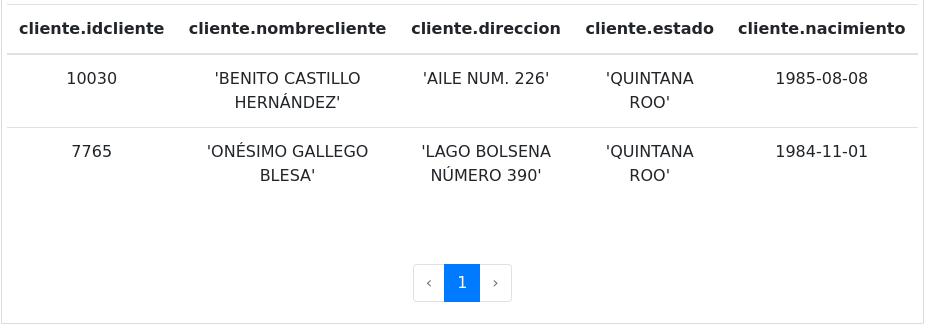
\includegraphics[width=17cm]{imgs/2a.png}
			\centering
		\end{figure}			
		\end{center}


		\newpage
		\item Obtener una relación de los clientes que \textbf{tienen una cuenta} con un saldo entre \textbf{\$85,000.00} y \textbf{\$115,000.00}, pero que \textbf{no tienen ningún préstamo} en el banco. Mostrar el \textbf{idcliente}, \textbf{nombre del cliente}, \textbf{número de cuenta} y \textbf{saldo}.\\\\
		Cuentas $=$ ctacliente $\bowtie$ $\sigma$ (saldo $\geqslant$ 85000.00 $\wedge$ saldo $\leqslant$ 115000.00) (cuenta)\\
		ClientesConPrestamos $=$ $\pi$ idcliente (prestatario)\\
		ClientesSinPrestamos $=$ $\pi$ idcliente (Cuentas) $-$ ClientesConPrestamos\\
		InfoClientes $=$ cliente $\bowtie$ ClientesSinPrestamos $\bowtie$ Cuentas\\
		$\pi$ idcliente, nombrecliente, numcta, saldo (InfoClientes)\\
		\begin{center}
		\begin{figure}[h!]
			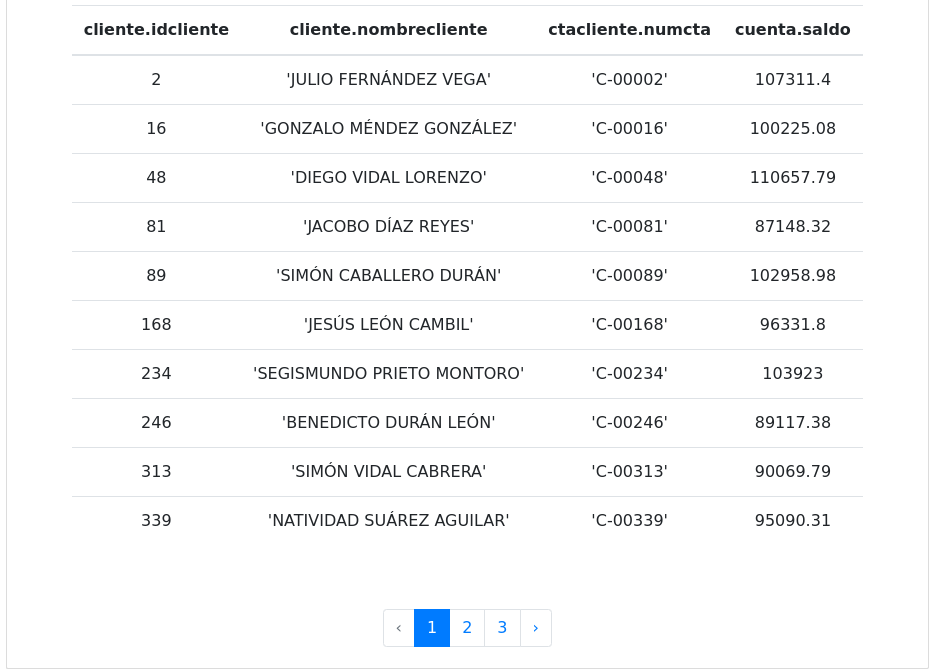
\includegraphics[width=17cm]{imgs/2b.png}
			\centering
		\end{figure}	
		\end{center}
		
		
		\newpage
		\item Obtener el \textbf{nombre} de todos los clientes que tienen \textbf{un préstamo} y el \textbf{importe} de este. El \textbf{importe} debe ser mayor de \textbf{\$95,000} y se debió entregar durante el \textbf{segundo trimestre de 2014} en el estado de \textbf{OAXACA}.\\\\
		SucursalesEnOaxaca $=$ $\sigma$ estado $=$ 'OAXACA' (sucursal)\\
		Prestamos $=$ $\sigma$ importe $>$ 95000.00 $\wedge$ fecha $\geqslant$ date('2014-04-01') $\wedge$ fecha $\leqslant$ date('2014-06-30') (prestamo)\\
		PrestamosEnOaxaca $=$ $\pi$ numprestamo, importe (SucursalesEnOaxaca $\bowtie$ Prestamos)\\
		ClientesConPrestamosEnOaxaca $=$ prestatario $\bowtie$ PrestamosEnOaxaca\\
		$\pi$ nombrecliente, importe (cliente $\bowtie$ ClientesConPrestamosEnOaxaca)\\
		\begin{center}
		\begin{figure}[h!]
			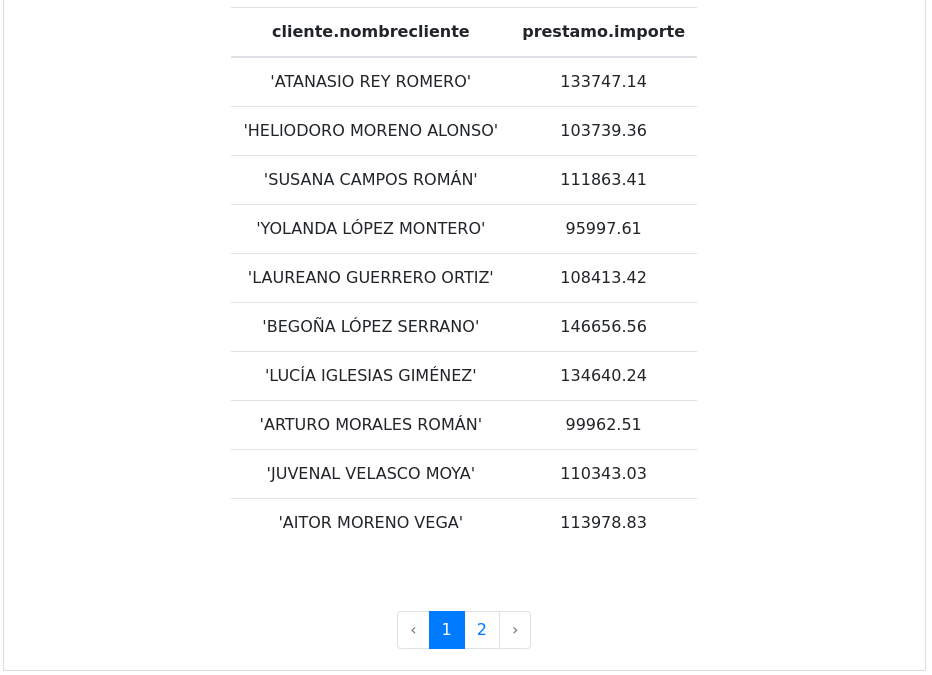
\includegraphics[width=17cm]{imgs/2c.png}
			\centering
		\end{figure}	
		\end{center}
		
		
		\newpage
		\item Toda la información de las sucursales con clientes que tengan un préstamo otorgado en el banco en alguna de las sucursales de \textbf{YUCATÁN} y que no vivan en \textbf{NAYARIT}.\\\\
		SucursalesEnYucatan $=$ $\sigma$ estado $=$ 'YUCATÁN' (sucursal)\\
		PrestamosFueraDeNayarit $=$ $\sigma$ estado $\neq$ 'NAYARIT' (cliente) $\bowtie$ prestatario $\bowtie$ prestamo\\
		$\pi$ numsucursal (PrestamosFueraDeNayarit) $\bowtie$ SucursalesEnYucatan\\
		\begin{center}
		\begin{figure}[h!]
			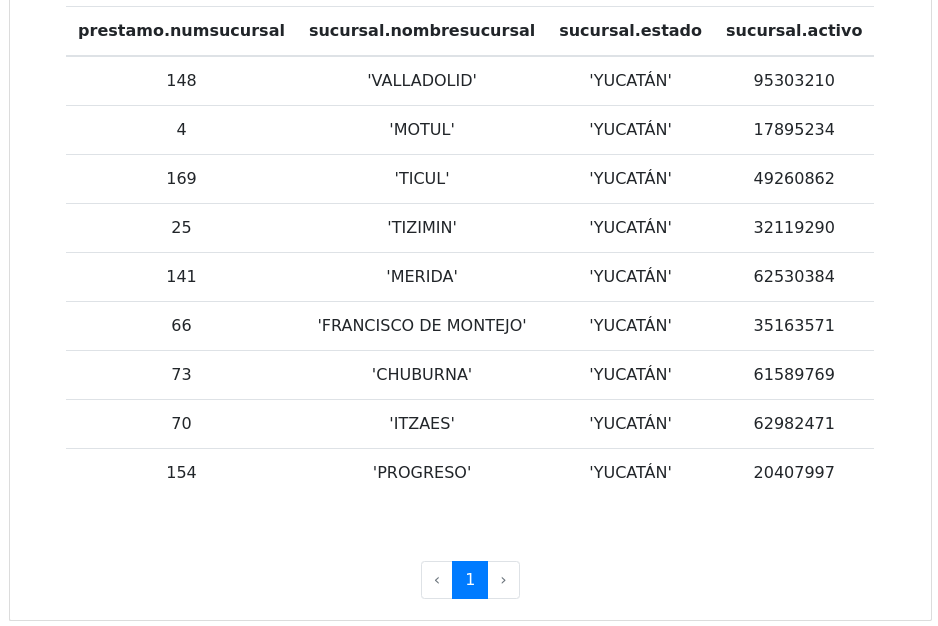
\includegraphics[width=17cm]{imgs/2d.png}
			\centering
		\end{figure}	
		\end{center}
		
		
		\newpage
		\item Toda la información de los clientes que solo tiene algún \textbf{préstamo} (ninguna cuenta) entregado en el \textbf{primer trimestre de 2013} y aquellos que solo tienen alguna \textbf{cuenta} (ningún préstamo) entregada durante el \textbf{segundo trimestre de 2014}.\\\\
		ClientesConPrestamosSinCuenta $=$ $\pi$ idcliente (prestatario $\bowtie$ $\sigma$ fecha $\geqslant$ date('2013-01-01') $\wedge$ fecha $\leqslant$ date('2013-03-31') (prestamo)) $-$ $\pi$ idcliente (ctacliente)\\
		ClientesConCuentasSinPrestamo $=$  $\pi$ idcliente (ctacliente $\bowtie$ $\sigma$ fecha $\geqslant$ date('2014-04-01') $\wedge$ fecha $\leqslant$ date('2014-06-30') (cuenta)) $-$ $\pi$ idcliente (prestatario)\\
		Total $=$ ClientesConPrestamosSinCuenta $\cup$ ClientesConCuentasSinPrestamo\\
		cliente $\bowtie$ Total\\
		\begin{center}
		\begin{figure}[h!]
			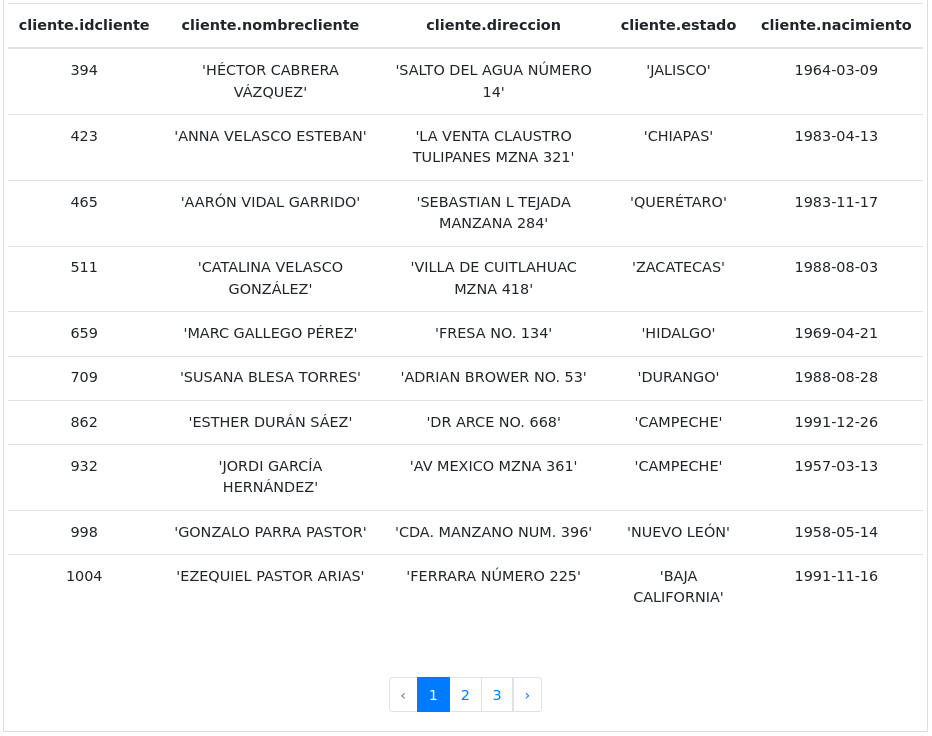
\includegraphics[width=17cm]{imgs/2e.png}
			\centering
		\end{figure}	
		\end{center}
		
		
		\newpage
		\item Una lista que muestre el \textbf{estado}, el \textbf{nombre de la sucursal} y el \textbf{total de clientes} que se tienen, considerando que los clientes deben tener una \textbf{cuenta} con saldo entre \textbf{\$90,000} y \textbf{\$120,000}, entregada en \textbf{2012} o \textbf{2014}.\\\\
		CuentasFecha $=$ $\sigma$ (fecha $\geqslant$ date('2012-01-01') $\wedge$ fecha $\leqslant$ date('2012-12-31')) $\vee$ (fecha $\geqslant$ date('2014-01-01') $\wedge$ fecha $\leqslant$ date('2014-12-31')) (cuenta)\\
		CuentasSaldo $=$ $\sigma$ saldo $\geqslant$ 90000.00 $\wedge$ saldo $\leqslant$ 120000.000 (CuentasFecha)\\
		CuentasCliente $=$ $\pi$ idcliente,numsucursal (ctacliente $\bowtie$ CuentasSaldo)\\
		ClientesSucursal $=$ $\gamma$ numsucursal ; count(idcliente) $\longrightarrow$ totalclientes (CuentasCliente)\\
		$\pi$ estado, nombresucursal, totalclientes (sucursal $\bowtie$ ClientesSucursal)\\
		\begin{center}
		\begin{figure}[h!]
			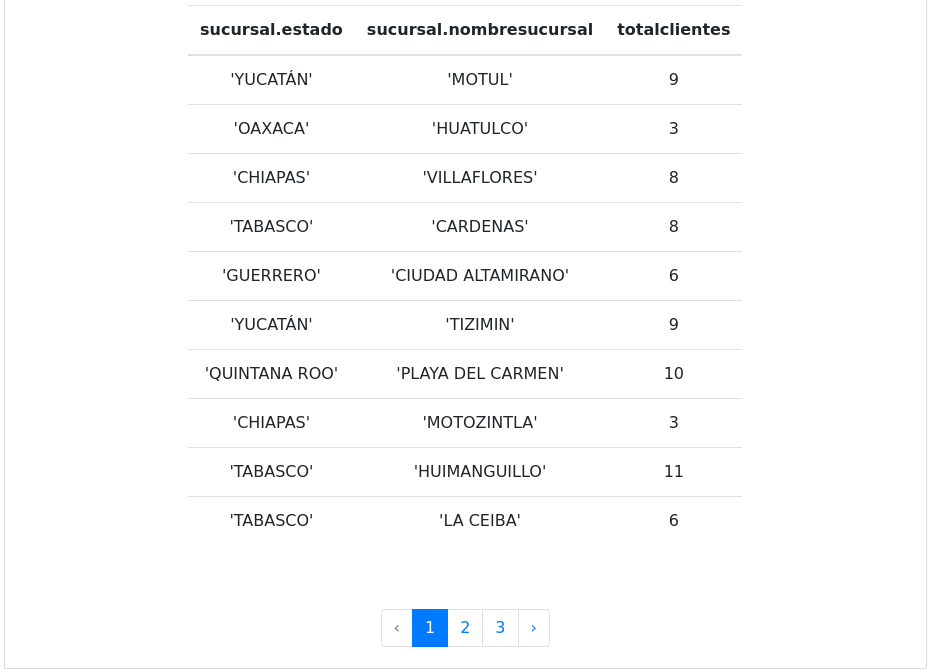
\includegraphics[width=17cm]{imgs/2f.png}
			\centering
		\end{figure}	
		\end{center}
		
		
		\newpage
		\item Información de los clientes con \textbf{saldo} entre \textbf{\$30,000.00} y \textbf{\$45,000.00} que vivan no vivan en \textbf{GUERRERO} y que no han solicitado ningún \textbf{préstamo}.\\\\
		ClientesFueraDeGuerrero $=$ $\sigma$ estado $\neq$ 'GUERRERO' (cliente)\\
		CuentasSaldo $=$ $\sigma$ saldo $\geqslant$ 30000.00 $\wedge$ saldo $\leqslant$ 45000.00 (cuenta)\\
		Clientes $=$ $\pi$ idcliente (ctacliente $\bowtie$ CuentasSaldo)\\
		ClientesSinPrestamo $=$ Clientes $-$ $\pi$ idcliente (prestatario)\\
		ClientesFueraDeGuerrero $\bowtie$ ClientesSinPrestamo\\
		\begin{center}
		\begin{figure}[h!]
			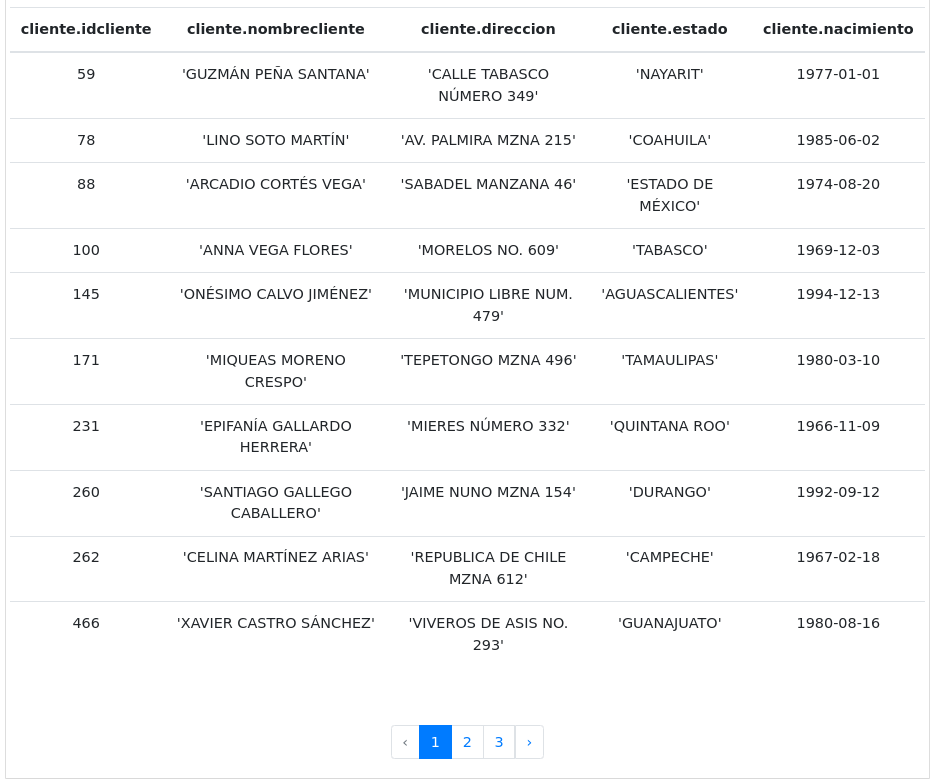
\includegraphics[width=17cm]{imgs/2g.png}
			\centering
		\end{figure}	
		\end{center}
		
		
		\newpage
		\item Una lista con el \textbf{saldo promedio, mayor saldo, menor saldo, y total de cuentas}, por \textbf{estado} y \textbf{sucursal}. El \textbf{saldo promedio} debe ser \textbf{mayor} que \textbf{\$80,000.00} y \textbf{menor} que \textbf{\$100,000.00} de los estados de \textbf{TABASCO, YUCATÁN Y QUINTANA ROO}.\\\\
		CuentasSucursal $=$ ctacliente $\bowtie$ cuenta $\bowtie$ sucursal\\
		SaldoPromSuc $=$ $\gamma$ numsucursal ; avg(saldo) $\longrightarrow$ promediosucursal (CuentasSucursal)\\
		CuentasSaldo $=$ CuentasSucursal $\bowtie$ SaldoPromSuc\\
		CuentasNoValidas $=$ $\sigma$ ((promediosucursal $<$ 80000.00 $\vee$ promediosucursal $>$ 100000.00) $\wedge$ (estado $=$ 'TABASCO' $\vee$ estado $=$ 'YUCATÁN' $\vee$ estado $=$ 'QUINTANA ROO')) (CuentasSaldo)\\
		CuentasValidas $=$ CuentasSaldo $-$ CuentasNoValidas\\
		MayorSaldoSuc $=$ $\gamma$ numsucursal ; max(saldo) $\longrightarrow$ mayorsaldo (CuentasValidas)\\
		MenorSaldoSuc $=$ $\gamma$ numsucursal ; min(saldo) $\longrightarrow$ menorsaldo (CuentasValidas)\\
		TotalCuentasSuc $=$ $\gamma$ numsucursal ; count(numcta) $\longrightarrow$ cuentassucursal (CuentasValidas)\\
		$\pi$ estado, nombresucursal, promediosucursal, mayorsaldo, menorsaldo, cuentassucursal (CuentasValidas $\bowtie$ MayorSaldoSuc $\bowtie$ MenorSaldoSuc $\bowtie$ TotalCuentasSuc)\\
		\begin{center}
		\begin{figure}[h!]
			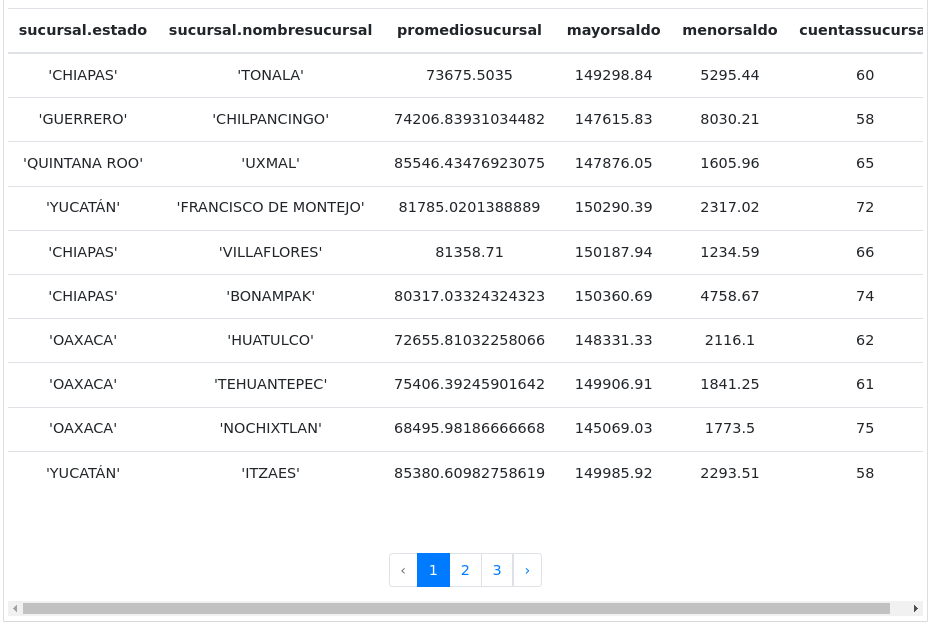
\includegraphics[width=17cm]{imgs/2h.png}
			\centering
		\end{figure}	
		\end{center}
		
		\newpage
		\item El estado que ha otorgado la \textbf{menor cantidad de préstamos}, cuyo importe esté entre \textbf{\$75,000.00} y \textbf{\$90,000.00}. Se debe mostrar también el \textbf{total de préstamos} que haya entregado.\\\\
		Prestamos $=$ $\sigma$ importe $\geqslant$ 75000.00 $\wedge$ importe  $\leqslant$ 90000.00 (prestamo)\\
		PrestamosSucursal $=$ Prestamos $\bowtie$ sucursal\\
		TotalPrestamosEstado $=$ $\gamma$ estado; count(numprestamo) $\longrightarrow$ totalprestamos (PrestamosSucursal)\\
		Min $=$ $\gamma$ min(totalprestamos) $\longrightarrow$ menorcantidadprestamos  (TotalPrestamosEstado)\\
		TotalPrestamosEstado $\bowtie$ (menorcantidadprestamos $=$ totalprestamos)  Min\\
		\begin{center}
		\begin{figure}[h!]
			
\includegraphics[width=17cm]{imgs/2i.png}
			\centering
		\end{figure}	
		\end{center}
		
		
		\newpage
		\item El \textbf{id}, \textbf{nombre del cliente}, \textbf{sucursal} y \textbf{saldo} de aquel cliente que tenga el \textbf{mayor importe} de todos los préstamos del
banco.\\\\
		ClientesSucursal $=$ cliente $\bowtie$ prestatario $\bowtie$ prestamo $\bowtie$ sucursal\\
		Max $=$ $\gamma$ max(importe) $\longrightarrow$ mayorimporte (ClientesSucursal)\\
		Total $=$ ClientesSucursal $\bowtie$ (mayorimporte $=$ importe) Max\\
		$\pi$ idcliente, nombrecliente, nombresucursal, importe (Total)\\
		\begin{center}
		\begin{figure}[h!]
			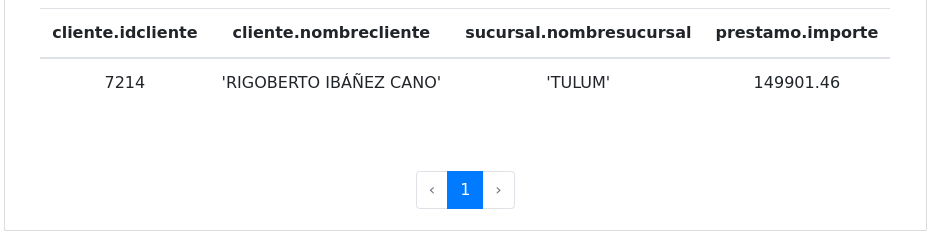
\includegraphics[width=17cm]{imgs/2j.png}
			\centering
		\end{figure}	
		\end{center}
		

	\end{enumerate}
	
	
	\newpage
	\textbf{Operaciones de mantenimiento de datos: borrado, inserción y actualización}
	\begin{enumerate}[label=\alph*.]
		\item Borrar toda la información del cliente \textbf{EDMUNDO RUBIO MONTERO}.\\\\
		Se busca la información de cuentas del cliente \textbf{EDMUNDO RUBIO MONTERO}. En este caso particular solo existe un cliente con dicho nombre.\\\\
		$\sigma$ nombrecliente $=$ 'EDMUNDO RUBIO MONTERO' (cliente $\bowtie$ ctacliente $\bowtie$ cuenta)
		\begin{center}
		\begin{figure}[h!]
			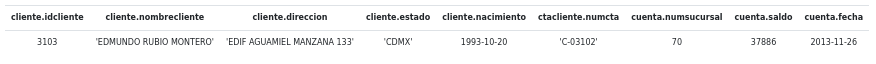
\includegraphics[width=17cm]{imgs/a1.png}
			\centering
		\end{figure}	
		\end{center}
		Esta información se guarda en una relación temporal y se utiliza para remover los datos de cuenta y ctacliente en ese orden.\\\\
		r = $\sigma$ nombrecliente = 'EDMUNDO RUBIO MONTERO' (cliente $\bowtie$ ctacliente $\bowtie$ cuenta)\\
cuenta1 $=$ cuenta $-$ ($\pi$ numcta,numsucursal,saldo,fecha (r))\\
ctacliente1 $=$ ctacliente $-$ ($\pi$ numcta,idcliente (r))\\

		Se usa una relación temporal para poder simular la operación en RelaX, estas relaciones para simular llevan el sufijo 1, por ejemplo cuenta1 es la relación que representa a cuenta sin el registro de la cuenta correspondiente a EDMUNDO RUBIO MONTERO.\\
		
		Análogamente se remueve la información de EDMUNDO RUBIO MONTERO de las relaciones prestamo y prestatario.\\
		
		s $=$ $\sigma$ nombrecliente $=$ 'EDMUNDO RUBIO MONTERO' (cliente $\bowtie$ prestatario $\bowtie$ prestamo)\\
prestamo1 $=$ prestamo $-$ ($\pi$ numprestamo,numsucursal,importe,fecha (s))\\
prestatario1 $=$ prestatario $-$ ($\pi$ numprestamo,idcliente (s))\\

		Finalmente se borra la información de la relación cliente, para ello se hace una reunión natural de cliente con la proyección de idcliente de la relación temporal r y este resultado se remueve de la relación cliente.\\
		
		cliente1 $=$ cliente $-$ (cliente $\bowtie$ ($\pi$ idcliente (r)))\\

		Para verificar buscamos la información de EDMUNDO RUBIO MONTERO con ayuda de las relaciones temporales r y s.
		
		(cuenta1 $\bowtie$ ($\pi$ numcta (r)))
		\begin{center}
		\begin{figure}[h!]
			
\includegraphics[width=12cm]{imgs/a2.png}
			\centering
		\end{figure}	
		\end{center}
		
		(ctacliente1 $\bowtie$ ($\pi$ idcliente (r)))
		\begin{center}
		\begin{figure}[h!]
			
\includegraphics[width=7cm]{imgs/a3.png}
			\centering
		\end{figure}	
		\end{center}
		
		(prestamo1 $\bowtie$ ($\pi$ numprestamo (s)))
		\begin{center}
		\begin{figure}[h!]
			
\includegraphics[width=14cm]{imgs/a4.png}
			\centering
		\end{figure}	
		\end{center}
		
		(prestatario1 $\bowtie$ ($\pi$ idcliente (s)))
		\begin{center}
		\begin{figure}[h!]
			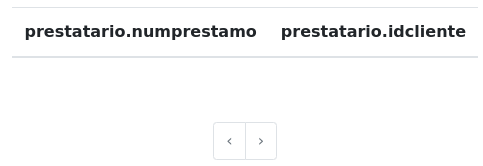
\includegraphics[width=8cm]{imgs/a5.png}
			\centering
		\end{figure}	
		\end{center}
		
		(cliente1 $\bowtie$ ($\pi$ idcliente (s)))
		\begin{center}
		\begin{figure}[h!]
			
\includegraphics[width=16cm]{imgs/a6.png}
			\centering
		\end{figure}	
		\end{center}
		
		Como se puede observar toda la información del cliente EDMUNDO RUBIO MONTERO fue eliminada.
		
		
		\newpage
		\item Borrar todas las cuentas de la sucursal \textbf{CHILPANCINGO} con un \textbf{saldo} entre \textbf{\$75,000.00} y \textbf{\$90,000.00}.\\\\
		Para esto se obtienen las cuentas de sucursal CHILPANCINGO, se filtran por el saldo y se hace una reunión natural con ctacliente. La información resultante en la relación temporal s se utiliza para remover las tuplas de ctacliente y cuenta.\\
		
		r $=$ $\sigma$ nombresucursal = 'CHILPANCINGO' (sucursal $\bowtie$ cuenta)\\
s $=$ ($\sigma$ saldo $\geqslant$ 75000 $\wedge$ saldo $\leqslant$ 90000 (r)) $\bowtie$ ctacliente\\
ctacliente1 $=$ ctacliente $-$ ($\pi$ numcta,idcliente (s))\\
cuenta1 $=$ cuenta $-$ ($\pi$ numcta,numsucursal,saldo,fecha (s))\\
		
		Se comprueba que se eliminaron las cuentas:
		cuenta1 $\bowtie$ ($\pi$ numcta (s))
		\begin{center}
		\begin{figure}[h!]
			
\includegraphics[width=16cm]{imgs/b1.png}
			\centering
		\end{figure}	
		\end{center}
		
		
		\newpage
		\item Ofrecer un nuevo préstamo con \textbf{\$20,000.00} a todos los clientes que tienen cuenta con saldo mayor de \textbf{\$60,000.00} y menor de \textbf{\$75,000.00} en la sucursal \textbf{BONAMPAK}, el número del nuevo préstamo será el de la cuenta que poseen. A los clientes con un saldo es mayor o igual a \textbf{\$75,000.00}, se les otorgará un préstamo de \textbf{\$30,000.00}.
		
		\newpage
		\item Aumentar todos los saldos de la sucursal \textbf{CARDENAS} en un \textbf{8\%}.\\\\
		\begin{center}
		\begin{figure}[h!]
			
\includegraphics[width=16cm]{imgs/d1.png}
			\centering
		\end{figure}	
		\end{center}
		\begin{center}
		\begin{figure}[h!]
			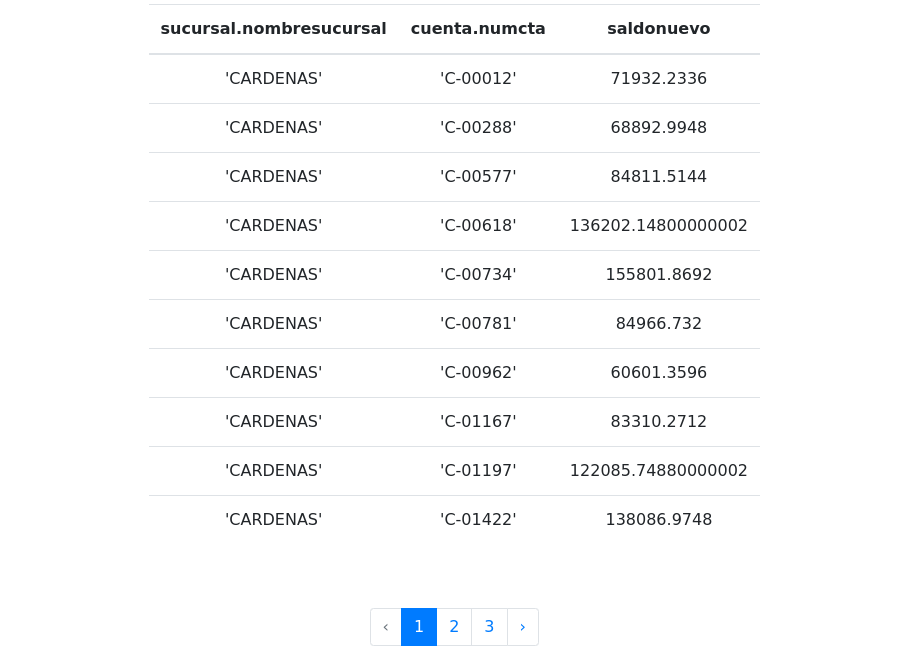
\includegraphics[width=16cm]{imgs/d2.png}
			\centering
		\end{figure}	
		\end{center}
		
		
		\newpage
		\item Disminuir \textbf{8\%} a las cuentas con saldo mayor a \textbf{\$90,000} y a las demás en un \textbf{4\%}. Las cuentas deben haber sido
entregadas en la sucursal \textbf{HUATULCO}.\\\\
		\begin{center}
		\begin{figure}[h!]
			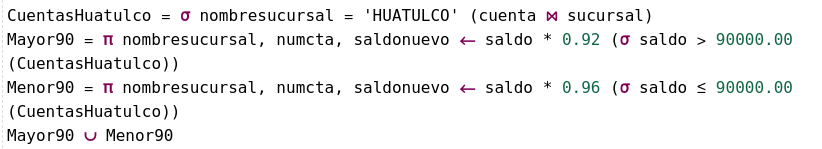
\includegraphics[width=16cm]{imgs/e1.png}
			\centering
		\end{figure}	
		\end{center}
		\begin{center}
		\begin{figure}[h!]
			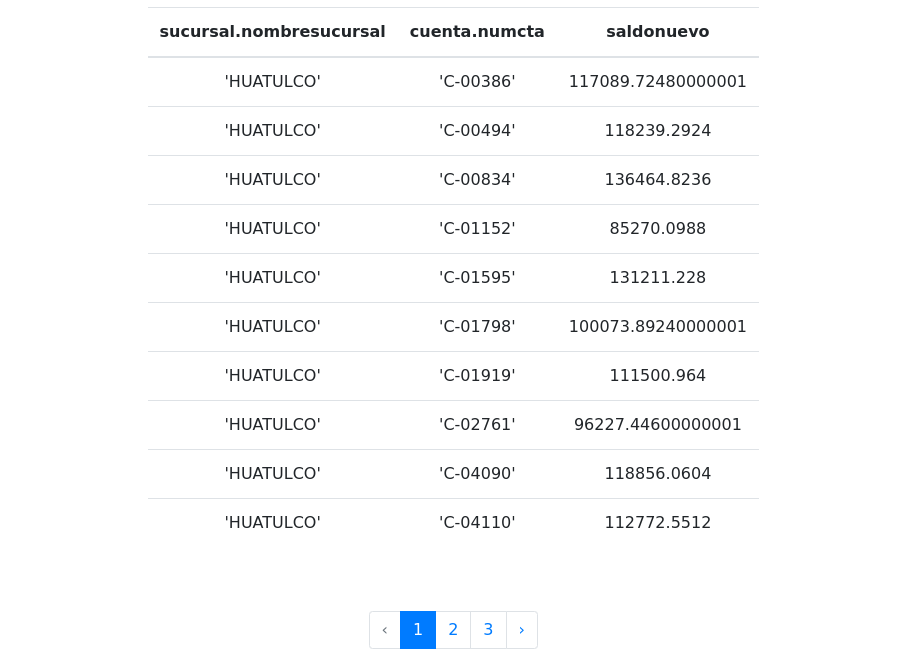
\includegraphics[width=16cm]{imgs/e2.png}
			\centering
		\end{figure}	
		\end{center}
	\end{enumerate}
	
	
\end{questions}

\end{document}
